\chapter{Chapter 3 - Design of MCM and MIMO Processing Systems for Urban Communication}

This chapter focuses on the algorithms implemented as part of the \acrshort{mcm} \acrshort{mimo} system. We look into the different aspects of transmitter block, channel parameters and receiver block. We look into the simulation of \acrshort{siso}, \acrshort{simo} ( transmit \gls{spatial diversity}), \acrshort{miso} (\acrshort{ostbc}) and \acrshort{mimo} ( both \gls{spatial diversity} and multiplexing(inverse channel decoding and \acrshort{svd})). 
 
\section{Basic Overview of our system}

The below figure shows the general block diagram of a communication system. We discuss all the blocks in great detain in this session.

\begin{figure}[!htbp]
\centering
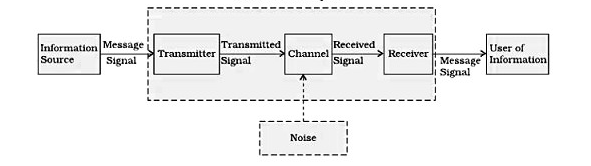
\includegraphics[scale=1]{Chapter 3/Figures/Block system}
\label{fig:general block digram}
\end{figure}

\section{Transmitter}

\subsection{PRBS Generator}
Here we explain the PRBS generator and the logic of our PRBS Code.

\subsection{Tone Loading Algorithm for the transmitter}
Here we explain in detail the tone loading algorithm (fine gains algorithm) which we have implemented in our code.

\subsection{QAM Modulator}
Here we explain the construction of the QAM modulator in detail and explain the recursive algorithm which we have used for the same.

\subsection{Alamouti Coder}
Here we explain the code relating to the Alamouti coder. We have already discussed the theory behind Alamouti codes, here we just explain our code which implements it.


\subsection{Inverse Channel Estimator and Coder}
In this section we discuss the implementation details of our Inverse Channel Estimation coder.


\subsection{Singular Value Decomposition Coder}
In this section we discuss the implementation details of our SVD coder. 

\section{Channel Parameters}

\subsection{AWGN Noise}
A small section explaining the AWGN noise that we are adding to our transmitted bit stream.

\subsection{Rayleigh Fading}
A small section discussing the implementation of Rayleigh Fading in our channel.

\subsection{Path Loss Function}
A section describing the path loss function we are using and the various components of the formula.


\section{Receiver}

\subsection{Alamouti Decoder}
Here we explain the workings of the Alamouti decoder.

\subsection{QAM Demodulator}
This section deals with the QAM Demodulator part of the receiver.


\section{Different Systems}
\subsection{SISO System}
Discusses the implementation of SISO system.

\subsection{MISO System}
Discusses the implementation of MISO system.

\subsection{SIMO System}
Discusses the implementation of SIMO systems.

\subsection{MIMO System}
Discusses the implementation of MIMO systems.
 